\documentclass[letterpaper]{article}
\usepackage[margin=1in]{geometry}
\usepackage{amsmath,amssymb}
\usepackage{lmodern}
\usepackage[T1]{fontenc}
\usepackage{tikz}
\usetikzlibrary{decorations.markings}

\newcommand{\aln}[1]{\begin{align*} #1 \end{align*}} %fast align

\tikzstyle{every node}=[circle, draw, fill=black!50, inner sep=0pt, minimum width=4pt]
\tikzset{->-/.style={decoration={
      markings,
      mark=at position .5 with {\arrow{>}}},postaction={decorate}}}
\tikzset{-<-/.style={decoration={
      markings,
      mark=at position .5 with {\arrow{<}}},postaction={decorate}}}

\begin{document}

\title{Gr\"obner Bases of Some Directed Graphs}
\author{Max Comstock}
\date{Summer 2014}
\maketitle

\section{Three Vertices with One Hamiltonian Cycle}
We will begin by examining simple graphs with a single Hamiltonian cycle. After finding Gr\"obner bases of such graphs with different numbers of vertices, a pattern appears. This is helpful because it allows us to characterize graphs with a single Hamiltonian cycle by the Gr\"obner basis of the generated polynomial system of equations. We begin with the smallest case, a graph with three vertices:
\begin{center}
  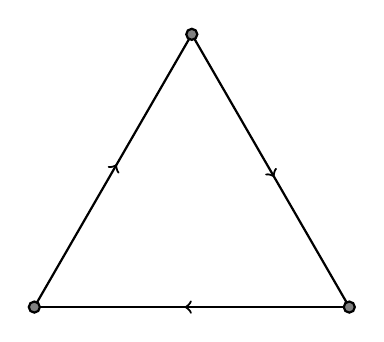
\begin{tikzpicture}[thick,scale=0.8]
    \draw[-<-] (0,0) to (5,0);
    \draw[-<-] (5,0) node{} to (60:5);
    \draw[-<-] (60:5) node{} to (0,0) node{};
  \end{tikzpicture}
\end{center}
The polynomial equations used to find Hamiltonian cycles are
\aln{
  z^2 + z + 1 &= 0\\
  x_i^3 - 1 &= 0 \quad 1 \leq i \leq 3\\
  z x_1 - x_2 &= 0\\
  z x_2 - x_3 &= 0\\
  z x_3 - x_1 &= 0
}
Using Macaulay2, we can find a reduced Gr\"obner basis for the ideal generated by these polynomials. We find
\aln{
  \{x_3^3-1, x_2-x_3z^2, x_1-x_3z\}
}
This is the same as
\aln{
  \{x_3^3-1, x_2+(z+1)x_3, x_1-zx_3\}
}

\newpage

\section{Four Vertices with One Hamiltonian Cycle}
We continue our investigation of simple graphs with a single Hamiltonian cycle. In this case, we will examine a graph with four vertices:
\begin{center}
  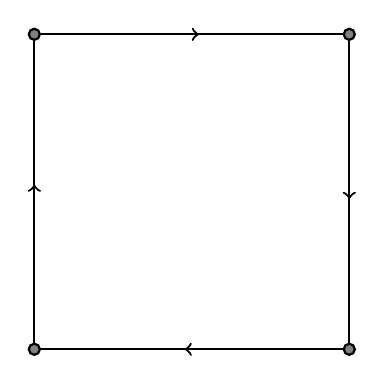
\begin{tikzpicture}[thick,scale=0.8]
    \draw[-<-] (0,0) -- (5,0);
    \draw[-<-] (5,0) node{} -- (5,5);
    \draw[-<-] (5,5) node{} -- (0,5);
    \draw[-<-] (0,5) node{} -- (0,0) node{};
  \end{tikzpicture}
\end{center}
The system of equations used to find Hamiltonian cycles for this graph is
\aln{
  z^2 + 1 &= 0\\
  x_i^4 - 1 &= 0 \quad 1 \leq i \leq 4\\
  z x_1 - x_2 &= 0\\
  z x_2 - x_3 &= 0\\
  z x_3 - x_4 &= 0\\
  z x_4 - x_1 &= 0
}
In this case, the reduced Gr\"bner basis of the ideal generated by the polynomial equations is
\aln{
  \{x_4^4-1, x_3-x_4z^3, x_2-x_4z^2, x_1-x_4z\}
}
This is the same as
\aln{
  \{x_4^4-1, x_3+zx_4, x_2+x_4, x_1-zx_4\}
}

\newpage

\section{Five Vertices with One Hamiltonian Cycle}
We continue our investigation of simple graphs with a single Hamiltonian cycle. In this case, we will examine a graph with five vertices:
\begin{center}
  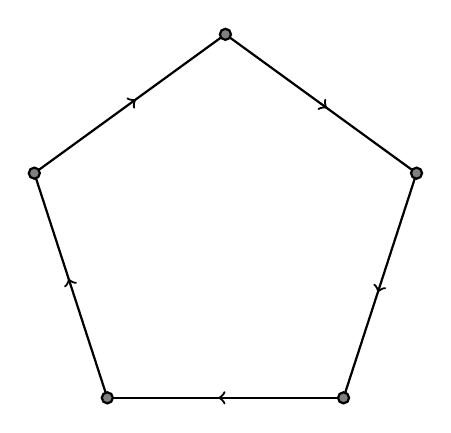
\begin{tikzpicture}[thick,scale=0.6]
    \draw[-<-] (0,0) -- (5,0);
    \draw[-<-] (5,0) node{} -- ++(72:5);
    \draw[-<-] (5,0)++(72:5) node{} -- ++(2*72:5);
    \draw[-<-] (5,0)++(72:5)++(2*72:5) node{} -- ++(3*72:5);
    \draw[-<-] (5,0)++(72:5)++(2*72:5)++(3*72:5) node{} -- (0,0) node{};
  \end{tikzpicture}
\end{center}
The system of equations used to find Hamiltonian cycles for this graph is
\aln{
  z^4 + z^3 + z^2 + z + 1 &= 0\\
  x_i^5 - 1 &= 0 \quad 1 \leq i \leq 5\\
  z x_1 - x_2 &= 0\\
  z x_2 - x_3 &= 0\\
  z x_3 - x_4 &= 0\\
  z x_4 - x_5 &= 0\\
  z x_5 - x_1 &= 0
}
Taking the reduced Gr\"obner basis of the ideal generated by the polynomial equations, we find
\aln{
  \{x_5^5-1, x_4-x_5z^4, x_3-x_5z^3, x_2-x_5z^2, x_1-x_5z\}
}
This is the same as
\aln{
  \{x_5^5-1, x_4+(z^3+z^2+z+1)x_5, x_3-z^3x_5, x_2-z^2x_5, x_1-zx_5\}
}

\newpage

\section{Six Vertices with One Hamiltonian Cycle}
For the last case of a simple graph with a single Hamiltonian cycle, we extend our results to graphs with six vertices. At this point, the pattern for such graphs with $n$ vertices is relatively clear.
\begin{center}
  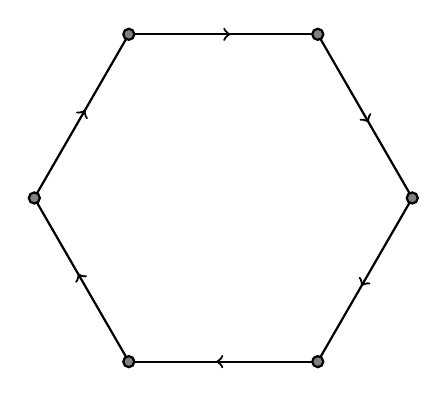
\begin{tikzpicture}[thick,scale=0.6]
    \draw[-<-] (0,0) -- (4,0);
    \draw[-<-] (4,0) node{} -- ++(60:4);
    \draw[-<-] (4,0)++(60:4) node{} -- ++(2*60:4);
    \draw[-<-] (4,0)++(60:4)++(2*60:4) node{} -- ++(3*60:4);
    \draw[-<-] (4,0)++(60:4)++(2*60:4)++(3*60:4) node{} -- ++(4*60:4);
    \draw[-<-] (4,0)++(60:4)++(2*60:4)++(3*60:4)++(4*60:4) node{} -- (0,0) node{};
  \end{tikzpicture}
\end{center}
The system of equations used to find Hamiltonian cycles for this graph is
\aln{
  z^2 - z + 1 &= 0\\
  x_i^6 - 1 &= 0 \quad 1 \leq i \leq 6\\
  z x_1 - x_2 &= 0\\
  z x_2 - x_3 &= 0\\
  z x_3 - x_4 &= 0\\
  z x_4 - x_5 &= 0\\
  z x_5 - x_6 &= 0\\
  z x_6 - x_1 &= 0
}
By taking the reduced Gr\"obner basis of the ideal generated by the polynomial equations, we find
\aln{
  \{x_6^6-1, x_5-x_6z^5, x_4-x_6z^4, x_3-x_6z^3, x_2-x_6z^2, x_1-x_6z\}
}
This is the same as
\aln{
  \{x_6^6-1, x_5+(z-1)x_6, x_4+zx_6, x_3+x_6, x_2+(-z+1)x_6, x_1-zx_6\}
}

\newpage

\section{Four Vertices with No Hamiltonian Cycles}
We will now examine a case where there are clearly no Hamiltonian cycles. Again, we will use a graph with four vertices, but this time the direction of the arcs does not allow a cycle to exist.
\begin{center}
  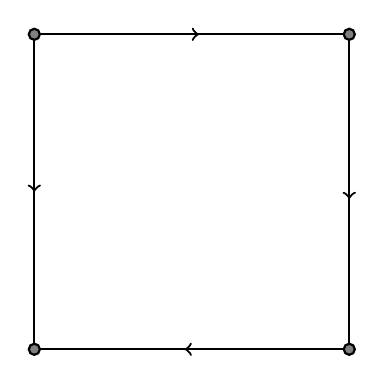
\begin{tikzpicture}[thick,scale=0.8]
    \draw[-<-] (0,0) -- (5,0);
    \draw[-<-] (5,0) node{} -- (5,5);
    \draw[-<-] (5,5) node{} -- (0,5);
    \draw[->-] (0,5) node{} -- (0,0) node{};
  \end{tikzpicture}
\end{center}
The polynomial system of equations used to find Hamiltonian cycles for this graph is
\aln{
  z^2 + 1 &= 0\\
  x_i^4 - 1 &= 0 \quad 1 \leq i \leq 4\\
  (z x_1 - x_2)(z x_1 - x_4) &= 0\\
  z x_2 - x_3 &= 0\\
  z x_3 - x_4 &= 0
}
We will now take the Gr\"obner basis of the ideal generated by these polynomials. We find
\aln{
  \{x_4^4-1, x_3-x_4z^3, x_2-x_4z^2, x_1z^2+x_1-x_4z^3-x_4z, x_1^2-x_4^2z^2\}
}
This is the same as
\aln{
  \{x_4^4-1, x_3+zx_4, x_2+x_4, x_1^2+x_4^2\}
}
Note that we find a solution, even though there are no Hamiltonian cycles. This is because this technique works only when every vertex has outdegree 1.

\newpage

\section{Five Vertices with One Hamiltonian Cycle and Additional Arcs}
This is an example of a graph with more arcs than necessary to have a single Hamiltonian cycle, but that still contains only one Hamiltonian cycle. We will compare this result with the previous graph that had five vertices and one Hamiltonian cycle, but did not have any additional arcs.
\begin{center}
  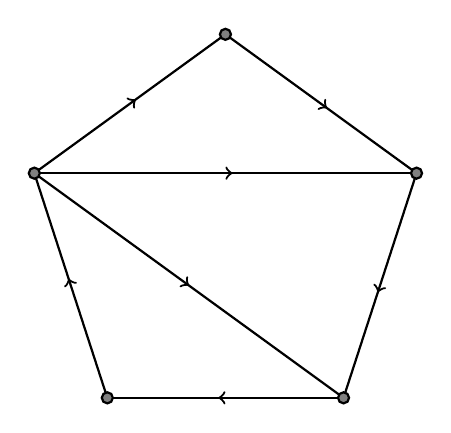
\begin{tikzpicture}[thick,scale=0.6]
    \draw[->-] (108:5) -- (5,0);
    \draw[-<-] (5,0) ++(72:5) -- (108:5);
    
    \draw[-<-] (0,0) -- (5,0);
    \draw[-<-] (5,0) node{} -- ++(72:5);
    \draw[-<-] (5,0)++(72:5) node{} -- ++(2*72:5);
    \draw[-<-] (5,0)++(72:5)++(2*72:5) node{} -- ++(3*72:5);
    \draw[-<-] (5,0)++(72:5)++(2*72:5)++(3*72:5) node{} -- (0,0) node{};
  \end{tikzpicture}
\end{center}
The system of equations used to find Hamiltonian cycles for this graph is
\aln{
  z^4 + z^3 + z^2 + z + 1 &= 0\\
  x_i^5 - 1 &= 0 \quad 1 \leq i \leq 5\\
  (z x_1 - x_2)(z x_1 - x_3)(z x_1 - x_4) &= 0\\
  z x_2 - x_3 &= 0\\
  z x_3 - x_4 &= 0\\
  z x_4 - x_5 &= 0\\
  z x_5 - x_1 &= 0
}
By taking the Gr\"obner basis of the ideal generated by these polynomials, we find
\aln{
  \{x_5^5-1, x_4-x_5z^4, x_3-x_5z^3, x_2-x_5z^2, x_1-x_5z\}
}
This is the same as
\aln{
  \{x_5^5-1, x_4+(z^3+z^2+z+1)x_5, x_3-z^3x_5, x_2-z^2x_5, x_1-zx_5\}
}

\newpage

\section{Five Verices with Multiple Hamiltonian Cycles}
In this case, we have a graph with 5 vertices and multiple Hamiltonian cycles. We would like to find consistent differences between graphs with two or more Hamiltonian cycles and graphs with fewer than two Hamiltonian cycles.
\begin{center}
  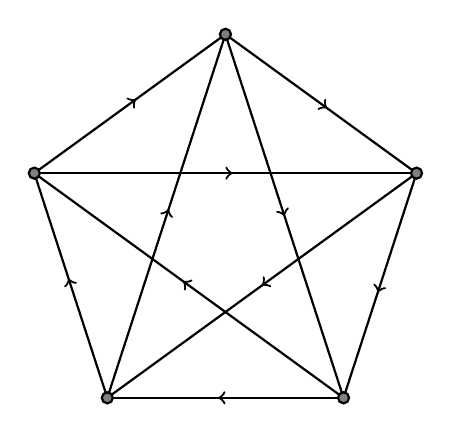
\begin{tikzpicture}[thick,scale=0.6]
    \draw[->-] (5,0)++(72:5) -- (0,0);
    \draw[-<-] (5,0)++(72:5)++(2*72:5) -- (0,0);
    \draw[->-] (5,0)++(72:5)++(2*72:5) -- (5,0);
    \draw[-<-] (108:5) -- (5,0);
    \draw[-<-] (5,0) ++(72:5) -- (108:5);
    \draw[-<-] (0,0) -- (5,0);
    \draw[-<-] (5,0) node{} -- ++(72:5);
    \draw[-<-] (5,0)++(72:5) node{} -- ++(2*72:5);
    \draw[-<-] (5,0)++(72:5)++(2*72:5) node{} -- ++(3*72:5);
    \draw[-<-] (5,0)++(72:5)++(2*72:5)++(3*72:5) node{} -- (0,0) node{};
  \end{tikzpicture}
\end{center}
The following system of equations characterizes the Hamiltonian cycles of the graph
\aln{
  z^4 + z^3 + z^2 + z + 1 &= 0\\
  x_i^5 - 1 &= 0 \quad 1 \leq i \leq 5\\
  (z x_1 - x_2)(z x_1 - x_3) &= 0\\
  (z x_2 - x_3)(z x_2 - x_4) &= 0\\
  (z x_3 - x_4)(z x_3 - x_5) &= 0\\
  (z x_4 - x_5)(z x_4 - x_1) &= 0\\
  (z x_5 - x_1)(z x_5 - x_2) &= 0
}
Now we can take the Gr\"obner basis of the ideal generated by these polynomials. The result is
\aln{
  \{& x_5^5-1, x_4^2+(z^3+z+1)x_4x_5+zx_5^2, x_3+(z^3+z+1)x_4+zx_5,\\& x_2+(z^2+1)x_4+(z^3+1)x_5, x_1+(-z^3-z^2-z-1)x_4+(-z^3-z)x_5\}
}

\newpage

\section{Six Vertices with Multiple Hamiltonian Cycles}
We will now examine a graph with six vertices and multiple Hamiltonian cycles.
\begin{center}
  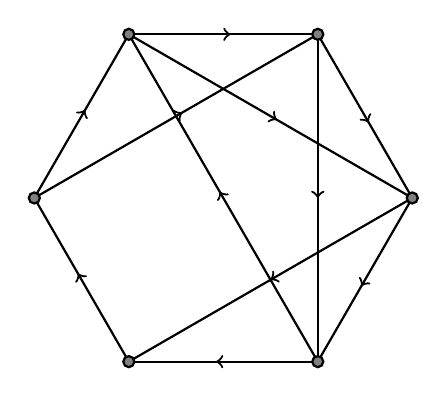
\begin{tikzpicture}[thick,scale=0.6]
    \draw[->-] (4,0)++(60:4) -- (0,0);
    \draw[-<-] (4,0)++(60:4)++(2*60:4)++(3*60:4) -- (4,0);
    \path (4,0)++(60:4)++(2*60:4)++(3*60:4) coordinate(farpoint);
    \draw[-<-] (4,0)++(60:4) -- (farpoint);
    \draw[->-] (4,0)++(60:4)++(2*60:4) -- (4,0);
    \draw[-<-] (4,0)++(60:4)++(2*60:4) -- (120:4);
    
    \draw[-<-] (0,0) -- (4,0);
    \draw[-<-] (4,0) node{} -- ++(60:4);
    \draw[-<-] (4,0)++(60:4) node{} -- ++(2*60:4);
    \draw[-<-] (4,0)++(60:4)++(2*60:4) node{} -- ++(3*60:4);
    \draw[-<-] (4,0)++(60:4)++(2*60:4)++(3*60:4) node{} -- ++(4*60:4);
    \draw[-<-] (4,0)++(60:4)++(2*60:4)++(3*60:4)++(4*60:4) node{} -- (0,0) node{};
  \end{tikzpicture}
\end{center}
We will use the following system of polynomial equations to examine the Hamiltonian cycles in the graph
\aln{
  z^2 - z + 1 &= 0\\
  x_i^6 - 1 &= 0 \quad 1 \leq i \leq 6\\
  (z x_1 - x_2)(z x_1 - x_3) &= 0\\
  (z x_2 - x_3)(z x_2 - x_4) &= 0\\
  (z x_3 - x_4)(z x_3 - x_5) &= 0\\
  (z x_4 - x_5)(z x_4 - x_1) &= 0\\
  z x_5 - x_6 &= 0\\
  (z x_6 - x_1)(z x_6 - x_2) &= 0
}
Now, we take the Gr\"obner basis of the ideal generated by these polynomials:
\aln{
  \{& x_6^6-1, x_5+(z-1)x_6, x_4^2+x_4x_6+x_6^2, 3x_3+(z+1)x_4+(2z+2)x_6,\\& 3x_2+(2z-1)x_4+(-2z+1)x_6, x_1+(-z+1)x_4+(-z+1)x_6\}
}

\newpage

\section{Six Vertices with Additional Chords}
This case has many arcs, but still only a single Hamiltonian cycle.
\begin{center}
  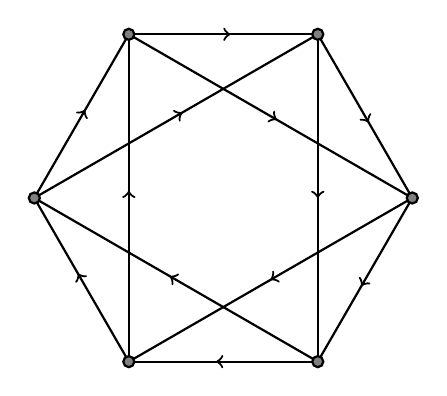
\begin{tikzpicture}[thick,scale=0.6]
    \draw[->-] (4,0)++(60:4) -- (0,0);
    \draw[-<-] (4,0)++(60:4)++(2*60:4)++(3*60:4) -- (0,0);
    \path (4,0)++(60:4)++(2*60:4)++(3*60:4) coordinate(farpoint);
    \draw[-<-] (4,0)++(60:4) -- (farpoint);
    \draw[->-] (4,0)++(60:4)++(2*60:4) -- (4,0);
    \draw[-<-] (4,0)++(60:4)++(2*60:4) -- (120:4);
    \draw[-<-] (120:4) -- (4,0);
    
    \draw[-<-] (0,0) -- (4,0);
    \draw[-<-] (4,0) node{} -- ++(60:4);
    \draw[-<-] (4,0)++(60:4) node{} -- ++(2*60:4);
    \draw[-<-] (4,0)++(60:4)++(2*60:4) node{} -- ++(3*60:4);
    \draw[-<-] (4,0)++(60:4)++(2*60:4)++(3*60:4) node{} -- ++(4*60:4);
    \draw[-<-] (4,0)++(60:4)++(2*60:4)++(3*60:4)++(4*60:4) node{} -- (0,0) node{};
  \end{tikzpicture}
\end{center}
This gives us the system
\aln{
  z^2 - z + 1 &= 0\\
  x_i^6 - 1 &= 0 \quad 1 \leq i \leq 6\\
  (z x_1 - x_2)(z x_1 - x_3) &= 0\\
  (z x_2 - x_3)(z x_2 - x_4) &= 0\\
  (z x_3 - x_4)(z x_3 - x_5) &= 0\\
  (z x_4 - x_5)(z x_4 - x_6) &= 0\\
  (z x_5 - x_6)(z x_5 - x_1) &= 0\\
  (z x_6 - x_1)(z x_6 - x_2) &= 0
}
The resulting Gr\"obner basis from the ideal generated by these polynomials is
\aln{
  \{x_6^6-1, x_5+(z-1)x_6, x_4+zx_6, x_3+x_6, x_2+(-z+1)x_6, x_1-zx_6\}
}

\newpage

\section{Previous Graph with Changed Arc Direction}
We now investigate a graph very similar to the previous case, but with the direction of some arcs reversed.
\begin{center}
  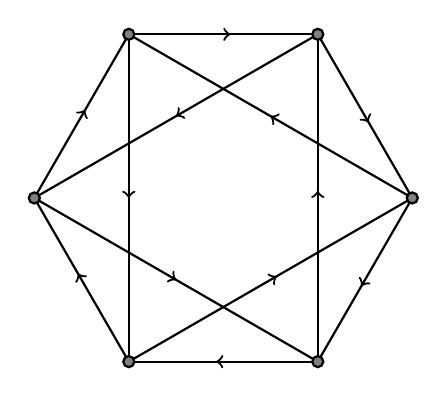
\begin{tikzpicture}[thick,scale=0.6]
    \draw[-<-] (4,0)++(60:4) -- (0,0);
    \draw[->-] (4,0)++(60:4)++(2*60:4)++(3*60:4) -- (0,0);
    \path (4,0)++(60:4)++(2*60:4)++(3*60:4) coordinate(farpoint);
    \draw[->-] (4,0)++(60:4) -- (farpoint);
    \draw[-<-] (4,0)++(60:4)++(2*60:4) -- (4,0);
    \draw[->-] (4,0)++(60:4)++(2*60:4) -- (120:4);
    \draw[->-] (120:4) -- (4,0);
    
    \draw[-<-] (0,0) -- (4,0);
    \draw[-<-] (4,0) node{} -- ++(60:4);
    \draw[-<-] (4,0)++(60:4) node{} -- ++(2*60:4);
    \draw[-<-] (4,0)++(60:4)++(2*60:4) node{} -- ++(3*60:4);
    \draw[-<-] (4,0)++(60:4)++(2*60:4)++(3*60:4) node{} -- ++(4*60:4);
    \draw[-<-] (4,0)++(60:4)++(2*60:4)++(3*60:4)++(4*60:4) node{} -- (0,0) node{};
  \end{tikzpicture}
\end{center}
We find the following system of polynomial equations from this graph
\aln{
  z^2 - z + 1 &= 0\\
  x_i^6 - 1 &= 0 \quad 1 \leq i \leq 6\\
  (z x_1 - x_2)(z x_1 - x_3) &= 0\\
  (z x_2 - x_3)(z x_2 - x_6) &= 0\\
  (z x_3 - x_4)(z x_3 - x_5) &= 0\\
  (z x_4 - x_5)(z x_4 - x_2) &= 0\\
  (z x_5 - x_6)(z x_5 - x_1) &= 0\\
  (z x_6 - x_1)(z x_6 - x_4) &= 0
}
Taking the Gr\"obner basis of the ideals generated by these polynomials, we find
\aln{
  \{x_6^6-1, x_5+(z-1)x_6, x_4+zx_6, x_3+x_6, x_2+(-z+1)x_6, x_1-zx_6\}
}

\newpage

\section{Four Vertices with Two Hamiltonian Cycles}
\begin{center}
  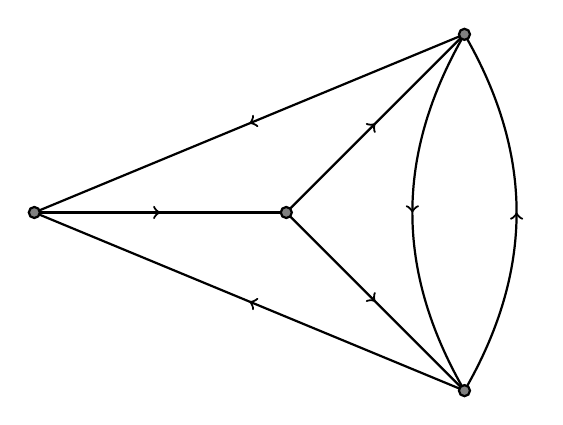
\begin{tikzpicture}[thick, scale=0.8]
    \path (4,0)++(45:4) coordinate(upper);
    \path (4,0)++(-45:4) coordinate(lower);
    \draw[->-] (upper) to (0,0);
    \draw[->-] (lower) to (0,0);
    \draw[->-] (upper) to[bend right] (lower);
    \draw[->-] (lower) to[bend right] (upper);
    \draw[->-] (0,0) node{} to (4,0);
    \draw[->-] (4,0) to ++(45:4) node{};
    \draw[->-] (4,0) node{} to ++(-45:4) node{};
  \end{tikzpicture}
\end{center}

\aln{
  x_i^4 - 1 &= 0 \quad 1 \leq i \leq 4\\
  z x_1 - x_2 &= 0\\
  (z x_2 - x_3) (z x_2 - x_4) &= 0\\
  (z x_3 - x_1) (z x_3 - x_4) &= 0\\
  (z x_4 - x_1) (z x_4 - x_3) &= 0
}

\aln{
  \{x_4^4-1, x_3^2+x_4^2, 2x_2+(z+1)x_3+(z+1)x_4, 2x_1+(-z+1)x_3+(-z+1)x_4\}
}

\newpage

\section{Five Vertex Extension of the Previous Graph}
\begin{center}
  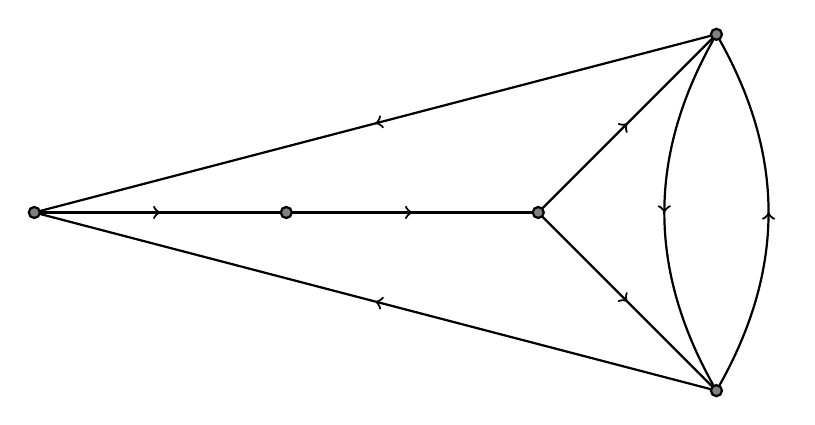
\begin{tikzpicture}[thick, scale=0.8]
    \path (4,0)++(45:4) coordinate(upper);
    \path (4,0)++(-45:4) coordinate(lower);
    \draw[->-] (upper) to (-4,0);
    \draw[->-] (lower) to (-4,0);
    \draw[->-] (upper) to[bend right] (lower);
    \draw[->-] (lower) to[bend right] (upper);
    \draw[->-] (-4,0) node{} to (0,0);
    \draw[->-] (0,0) node{} to (4,0);
    \draw[->-] (4,0) to ++(45:4) node{};
    \draw[->-] (4,0) node{} to ++(-45:4) node{};
  \end{tikzpicture}
\end{center}

\aln{
  x_i^5 - 1 &= 0 \quad 1 \leq i \leq 5\\
  z x_1 - x_2 &= 0\\
  z x_2 - x_3 &= 0\\
  (z x_3 - x_4) (z x_3 - x_5) &= 0\\
  (z x_4 - x_1) (z x_4 - x_5) &= 0\\
  (z x_5 - x_1) (z x_5 - x_4) &= 0
}

\aln{
  \{& x_5^5-1, x_4^2+(z^3+z^2+1)x_4x_5+x_5^2, x_3+(z^2+1)x_4+(z^2+1)x_5,\\& x_2+(-z^3-z^2-1)x_4+(-z^3-z^2-1)x_5, x_1+(z^3+1)x_4+(z^3+1)x_5\}
}

\newpage

\section{Five Vertices with Two Hamiltonian Cycles}
\begin{center}
  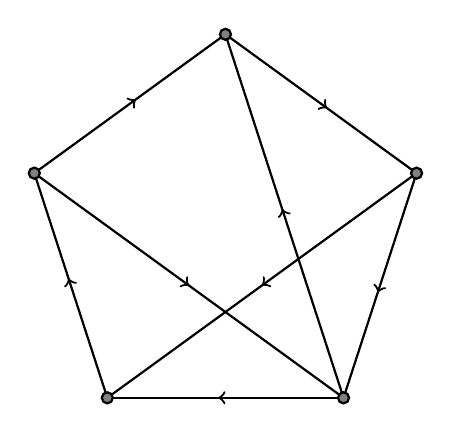
\begin{tikzpicture}[thick,scale=0.6]
    \draw[->-] (5,0)++(72:5) -- (0,0);
    \draw[-<-] (5,0)++(72:5)++(2*72:5) -- (5,0);
    \draw[->-] (108:5) -- (5,0);
    \draw[-<-] (0,0) -- (5,0);
    \draw[-<-] (5,0) node{} -- ++(72:5);
    \draw[-<-] (5,0)++(72:5) node{} -- ++(2*72:5);
    \draw[-<-] (5,0)++(72:5)++(2*72:5) node{} -- ++(3*72:5);
    \draw[-<-] (5,0)++(72:5)++(2*72:5)++(3*72:5) node{} -- (0,0) node{};
  \end{tikzpicture}
\end{center}

\aln{
  x_i^5 - 1 &= 0 \quad 1 \leq i \leq 5\\
  z x_1 - x_2 &= 0\\
  (z x_2 - x_3) (z x_2 - x_4) &= 0\\
  (z x_3 - x_1) (z x_3 - x_4) &= 0\\
  z x_4 - x_5 &= 0\\
  (z x_5 - x_1) (z x_5 - x_3) &= 0
}

\aln{
  \{& x_5^5-1, x_4+(z^3+z^2+z+1)x_5, x_3^2+(-z^3-z)x_3x_5+(-z^3-z^2-z-1)x_5^2,\\& x_2+(z^3+z+1)x_3+x_5, x_1+(-z^3-z)x_3+(-z^3-z^2-z-1)x_5\}
}

\newpage

\section{Six Vertices with Three Hamiltonian Cycles}
\begin{center}
  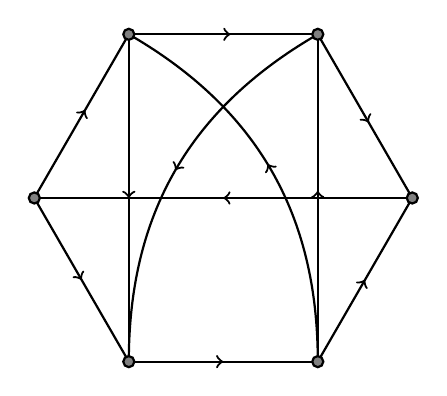
\begin{tikzpicture}[thick,scale=0.6]
    \path (4,0)++(60:4)++(2*60:4)++(3*60:4) coordinate(farpoint);
    \draw[->-] (4,0)++(60:4) -- (120:4);
    \draw[->-] (farpoint) -- (0,0);
    \draw[-<-] (4,0)++(60:4)++(2*60:4) -- (4,0);
    \draw[->-] (4,0)++(60:4)++(2*60:4) to[bend right] (0,0);
    \draw[-<-] (farpoint) to[bend left] (4,0);
    
    \draw[->-] (0,0) -- (4,0);
    \draw[->-] (4,0) node{} -- ++(60:4);
    \draw[-<-] (4,0)++(60:4) node{} -- ++(2*60:4);
    \draw[-<-] (4,0)++(60:4)++(2*60:4) node{} -- ++(3*60:4);
    \draw[-<-] (4,0)++(60:4)++(2*60:4)++(3*60:4) node{} -- ++(4*60:4);
    \draw[->-] (4,0)++(60:4)++(2*60:4)++(3*60:4)++(4*60:4) node{} -- (0,0) node{};
  \end{tikzpicture}
\end{center}

\aln{
  x_i^6 - 1 &= 0 \quad 1 \leq i \leq 6\\
  (z x_1 - x_2) (z x_1 - x_3) &= 0\\
  (z x_2 - x_3) (z x_2 - x_4) &= 0\\
  z x_3 - x_5 &= 0\\
  (z x_4 - x_3) (z x_4 - x_6) &= 0\\
  (z x_5 - x_2) (z x_5 - x_4) (z x_5 - x_6) &= 0\\
  z x_6 - x_1 &= 0
}

\aln{
  \{& x_6^6-1, x_5^3+2zx_5^2x_6+(2z-2)x_5x_6^2-x_6^3, x_4+x_5^2x_6^5+(z+1)x_5+(2z-1)x_6,\\& x_3+(z-1)x_5, x_2-x_5^2x_6^5+(-2z+1)x_5+(-z+2)x_6, x_1-zx_6\}
}

\newpage

\section{Five Vertices with Three Hamiltionian Cycles}
\begin{center}
  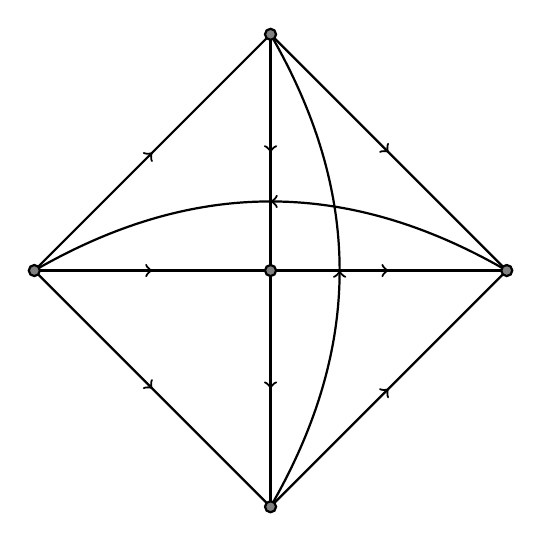
\begin{tikzpicture}[thick, scale=0.6]
    \draw[->-] (0,0) to (5,0);
    \draw[->-] (0,0) to (5,5);
    \draw[->-] (0,0) to (5,-5);
    \draw[->-] (5,5) to (5,0);
    \draw[->-] (5,0) to (5,-5);
    \draw[->-] (5,-5) to[bend right] (5,5);
    \draw[->-] (5,5) node{} to (10,0);
    \draw[->-] (5,0) node{} to (10,0);
    \draw[->-] (5,-5) node{} to (10,0);
    \draw[->-] (10,0) node{} to[bend right] (0,0) node{};
  \end{tikzpicture}
\end{center}

\aln{
  x_i^5 - 1 &= 0 \quad 1 \leq i \leq 5\\
  (z x_1 - x_2) (z x_1 - x_3) (z x_1 - x_4) &= 0\\
  (z x_2 - x_3) (z x_2 - x_5) &= 0\\
  (z x_3 - x_4) (z x_3 - x_5) &= 0\\
  (z x_4 - x_2) (z x_4 - x_5) &= 0\\
  z x_5 - x_1 &= 0
}

\aln{
  \{& x_5^5-1, x_4^3+(z+1)x_4^2x_5+(z^2+z+1)x_4x_5^2+(z^3+z^2+z+1)x_5^3,\\& 5x_3+(-z^3-2z^2-3z-4)x_4^2x_5^4+(2z^3-z^2+z+3)x_4+(-z^3-2z^2+2z+1)x_5,\\& 5x_2+(z^3+2z^2+3z+4)x_4^2x_5^4+(-2z^3+z^2-z+2)x_4+(z^3+2z^2+3z+4)x_5, x_1-zx_5\}
}

\newpage

\section{Six Vertices with Three Hamiltionian Cycles}
\begin{center}
  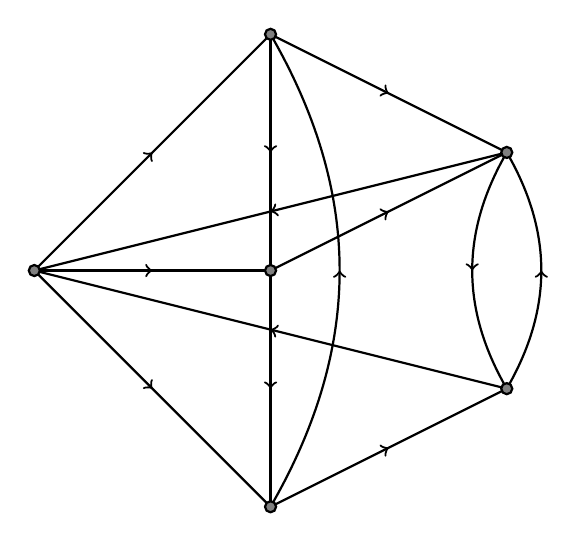
\begin{tikzpicture}[thick, scale=0.6]
    \draw[->-] (0,0) to (5,0);
    \draw[->-] (0,0) to (5,5);
    \draw[->-] (0,0) to (5,-5);
    \draw[->-] (5,5) to (5,0);
    \draw[->-] (5,0) to (5,-5);
    \draw[->-] (5,-5) to[bend right] (5,5);
    \draw[->-] (5,5) node{} to (10,2.5);
    \draw[->-] (5,0) node{} to (10,2.5);
    \draw[->-] (5,-5) node{} to (10,-2.5);
    \draw[->-] (10,2.5) to[bend right] (10,-2.5);
    \draw[->-] (10,-2.5) to[bend right] (10,2.5);
    \draw[->-] (10,2.5) node{} to (0,0);
    \draw[->-] (10,-2.5) node{} to (0,0) node{};
  \end{tikzpicture}
\end{center}

\aln{
  x_i^6 - 1 &= 0 \quad 1 \leq i \leq 6\\
  (z x_1 - x_2) (z x_1 - x_3) (z x_1 - x_4) &= 0\\
  (z x_2 - x_3) (z x_2 - x_5) &= 0\\
  (z x_3 - x_4) (z x_3 - x_5) &= 0\\
  (z x_4 - x_2) (z x_4 - x_6) &= 0\\
  (z x_5 - x_1) (z x_5 - x_6) &= 0\\
  (z x_6 - x_1) (z x_6 - x_5) &= 0
}

\aln{
  \{& x_6^6-1, x_5^2-x_5x_6+x_6^2, x_4x_5+(z-1)x_4x_6+(z-1)x_5x_6-zx_6^2, x_4^2+(-z+2)x_4x_6+2x_5x_6+(z-1)x_6^2,\\& x_3+(z+1)x_4+2zx_5, 3x_2-3zx_4+(-4z+2)x_5+(2z+2)x_6, 3x_1+(-2z+1)x_5+(-2z+1)x_6\}
}

\newpage

\section{Five Vertices with Two Hamiltonian Cycles}
\begin{center}
  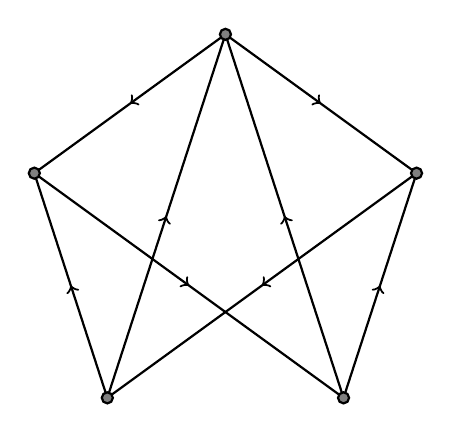
\begin{tikzpicture}[thick, scale=0.6]
    \path (5,0)++(72:5)++(2*72:5)++(3*72:5) coordinate(fifth);
    \path (5,0)++(72:5)++(2*72:5) coordinate(fourth);
    \path (5,0)++(72:5) coordinate(third);
    \draw[->-] (0,0) to (fifth);
    \draw[->-] (0,0) to (fourth);
    \draw[->-] (5,0) to (third);
    \draw[->-] (5,0) to (fourth);
    \draw[->-] (third) to (0,0) node{};
    \draw[->-] (fourth) to (third) node{};
    \draw[->-] (fourth) node{} to (fifth);
    \draw[->-] (fifth) node{} to (5,0) node{};
  \end{tikzpicture}
\end{center}

\aln{
  x_i^5 - 1 &= 0 \quad 1 \leq i \leq 5\\
  (z x_1 - x_2) (z x_1 - x_3) &= 0\\
  z x_2 - x_5 &= 0\\
  z x_3 - x_4 &= 0\\
  (z x_4 - x_1) (z x_4 - x_2) &= 0\\
  (z x_5 - x_1) (z x_5 - x_3) &= 0
}

\aln{
  \{& x_5^5-1, x_4^2+(-z^3-z^2)x_4x_5+x_5^2, x_3+(z^3+z^2+z+1)x_4, x_2+(z^3+z^2+z+1)x_5,\\& x_1+(-z^3-z^2-z)x_4+(-z^3-z^2-z)x_5\}
}

\newpage

\section{Five Vertices with Four Hamiltonian Cycles}
\begin{center}
  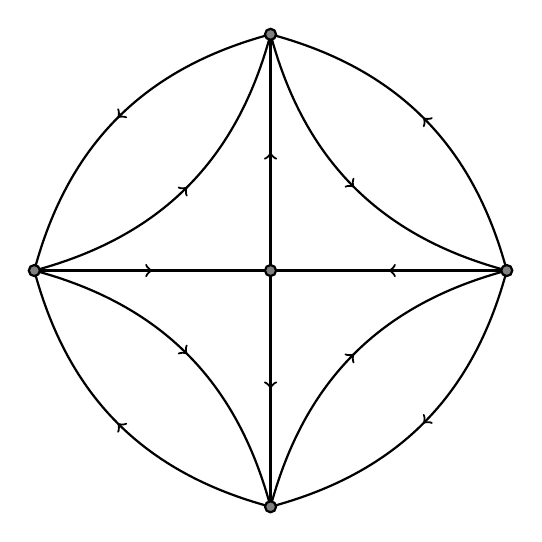
\begin{tikzpicture}[thick,scale=0.6]
    \draw[->-] (0,0) to (5,0);
    \draw[->-] (0,0) to[bend right] (5,5);
    \draw[->-] (0,0) to[bend left] (5,-5);
    \draw[->-] (5,0) to (5,5);
    \draw[->-] (5,0) to (5,-5);
    \draw[->-] (5,5) to[bend right] (0,0);
    \draw[->-] (5,5) to[bend right] (10,0);
    \draw[->-] (5,-5) to[bend left] (0,0) node{};
    \draw[->-] (5,-5) to[bend left] (10,0);
    \draw[->-] (10,0) to (5,0) node{};
    \draw[->-] (10,0) to[bend right] (5,5) node{};
    \draw[->-] (10,0) node{} to[bend left] (5,-5) node{};
  \end{tikzpicture}
\end{center}

\aln{
  x_i^5 - 1 &= 0 \quad 1 \leq i \leq 5\\
  (z x_1 - x_2) (z x_1 - x_3) (z x_1 - x_4) &= 0\\
  (z x_2 - x_1) (z x_2 - x_5) &= 0\\
  (z x_3 - x_2) (z x_3 - x_4) &= 0\\
  (z x_4 - x_1) (z x_4 - x_5) &= 0\\
  (z x_5 - x_2) (z x_5 - x_3) (z x_5 - x_4) &= 0
}

\aln{
	\{& x_5^5-1, x_4^3+(z^3+1)x_4^2x_5+(z^3+z+1)x_4x_5^2-z^2x_5^3,\\& x_3x_4+(z^3+z^2+z+1)x_3x_5+(z+1)x_4^2+(z^2+z+1)x_5^2, x_3^2+(-z^3-z)x_3x_5+(-z^3-z^2-z-1)x_5^2,\\& x_2+(-z^3-z)x_3+x_4, x_1+(z^3+z+1)x_3+x_5\}
}






\end{document}
